\subsection{Power Subsystem}
\label{sec:power_subsystem}
The power system is an important part to any electrical device or component that requires any amount of power. It simply starts from a power source such as a battery or wall outlet then is converted into energy to operate what is being used. At the minimum this model is designed to be an independent system, having the capability to operate on its own. The way that can be achieved is through solar power. \par
Solar power has been such a strong growing source of energy and will play a vital role in our system. Power is collected through the solar panels and then regulated through the charge controller. The power is regulated through the charge controller so that the battery is not being over charge, which could potentially damage it. Of course, power collected from the solar panels needs to be stored in a battery, which will also be used to power our system. From there, voltage needs to be regulated once more for the microcontroller and other components are powered properly. The block diagram in \autoref{fig:power-block-diagram} shows the flow of power through the system. 

\begin{figure}[H]
    \centering
    \caption{Power subsystem block diagram}
    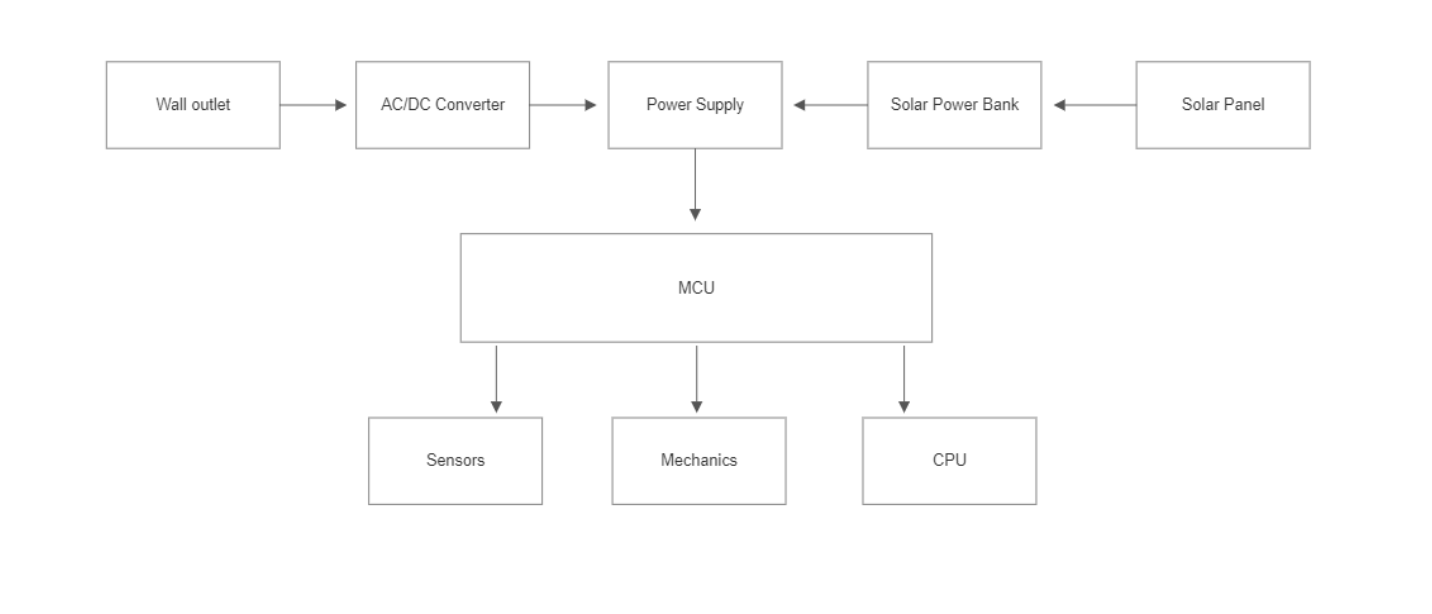
\includegraphics[width=\textwidth]{images/PowerSystemBlock.png}
    \label{fig:power-block-diagram}
\end{figure}
The block labeled ``Mechanics'' in \autoref{fig:power-block-diagram} refers to the solenoid valve for controlling water flow as well as the control scheme for actuating the solar panels to maximize power efficiency.
\subsubsection{Solar Panel Control}
To get a greater degree of accuracy the use of stepper motors are used. First, based on the choice of solar panels we get the mass and dimensions of the solar panels, these are .76kg and .336m x .2m respectively. This is important for calculating the torque. We only need to provide two degrees of freedom, one about the short axis (the horizontal axis that bisects the .2m side) and the vertical axis (the axis at the intersection that bisects the two sides of the panel). From the length and mass we can calculate the force per unit length:
\begin{equation}
    \frac{.76 \text{kg}}{.336 \text{m}}=22.62\frac{\text{N}}{\text{m}}
    \label{eqn:short-axis-fpl}
\end{equation}
Now, knowing that torque is $F\times d$ we can formulate the torque for any given angle about this axis in the following:
\begin{equation}
    \int_{0}^{.168} 22.62 \times x \times \sin{\theta} \, dx
    \label{eqn:short-axis-torque}
\end{equation}
\autoref{eqn:short-axis-torque} gives the torque for any given angle. Something you might have noticed is that this is for only one side of the panel. The full torque about the central axis is as follows:
\begin{equation}
    \int_{0}^{.168} 22.62 \times x \times \sin{\theta} \, dx - \int_{0}^{.168} 22.62 \times x \times \sin{180-\theta} \, dx
    \label{eqn:short-axis-torque-total}
\end{equation}
From \autoref{eqn:short-axis-torque-total} we can find the maximum and minimum values of the torque about the axis by finding the crossings of the first derivative with respect to $\theta$ and finding the concavity in the second derivate with respect to $\theta$. Doing so proves the intuition that there is no torque around either axis, this equation evaluates to 0 for all $\theta$.

To save on power \autoref{fig:stepper-config} shows that two motors will work to rotate the panels about the short axis while the center axis is actuated by a single motor and belt system.
\begin{figure}[H]
    \centering
    \caption{Stepper motor configuration}
    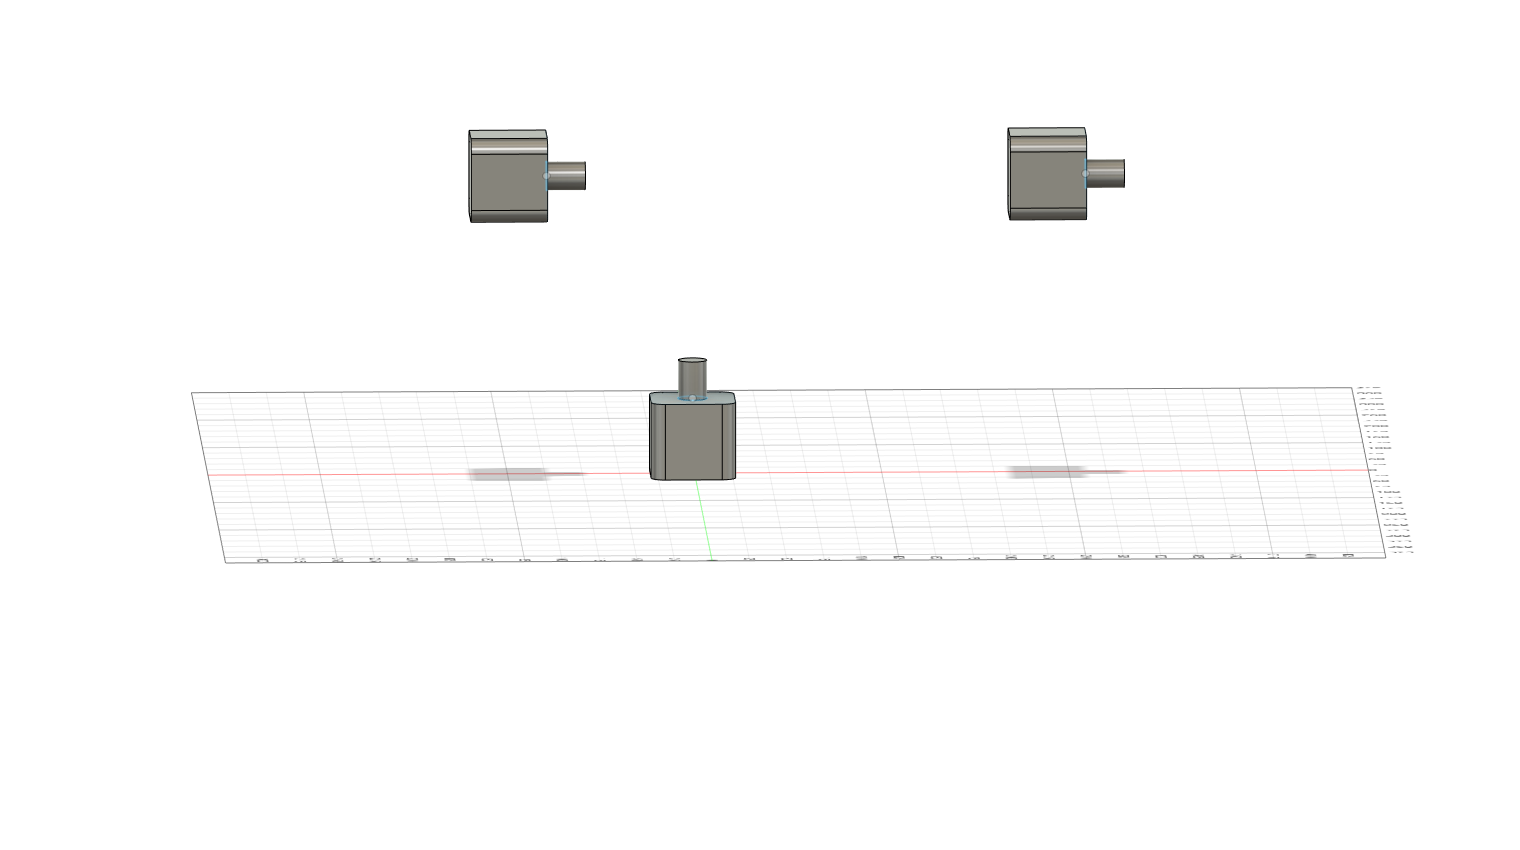
\includegraphics[width=0.5\textwidth]{images/stepper-config.png}
    \label{fig:stepper-config}
\end{figure}
The reason we have to use two stepper motors for the short axis rotation is that because as the panels rotate about their central axis any rod or pulley or tensioner system would come out of alignment. Another advantage of this due to the lack of torque in the system is that using a motor controller the two motors can be driven with a single H-bridge with a minimum penalty to power, this will ensure that both panels are always pointed at the same angle in the desired direction.